\newpage
\section{第 06 周}

\subsection{第 13 课 | 字典树和并查集}

\subsubsection{脑图}

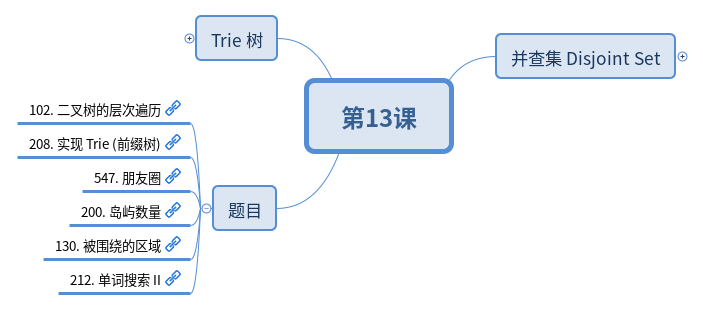
\includegraphics[width=140mm,height=60mm]{images/camp/第13课.png}

\subsubsection{题目}

\begin{itemize}
  \item \hyperref[leetcode:102]{102. 二叉树的层次遍历}
  \item \hyperref[leetcode:208]{208. 实现 Trie (前缀树)}
  \item \hyperref[leetcode:547]{547. 朋友圈}
  \item \hyperref[leetcode:200]{200. 岛屿数量}
  \item \hyperref[leetcode:130]{130. 被围绕的区域}
  \item \hyperref[leetcode:212]{212. 单词搜索 II}
\end{itemize}

\subsection{第 14 课 | 高级搜索}

\subsubsection{脑图}

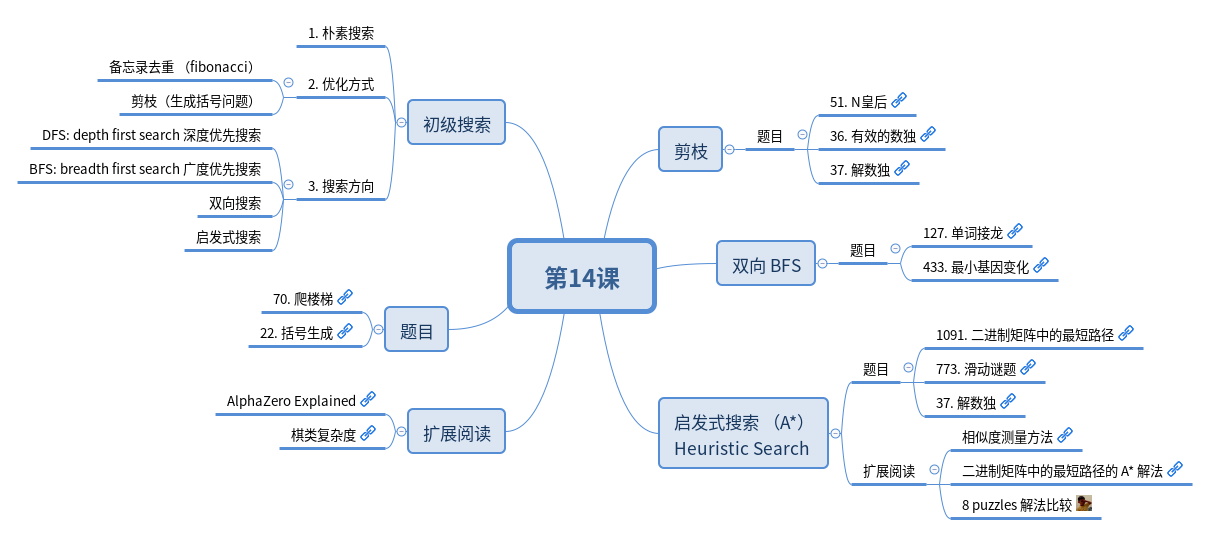
\includegraphics[width=140mm,height=60mm]{images/camp/第14课.png}

\subsubsection{题目}

\begin{itemize}
  \item \hyperref[leetcode:70]{70. 爬楼梯}
  \item \hyperref[leetcode:22]{22. 括号生成}
  \item \hyperref[leetcode:51]{51. N皇后}
  \item \hyperref[leetcode:36]{36. 有效的数独}
  \item \hyperref[leetcode:37]{37. 解数独}
  \item \hyperref[leetcode:127]{127. 单词接龙}
  \item \hyperref[leetcode:433]{433. 最小基因变化}
  \item \hyperref[leetcode:1091]{1091. 二进制矩阵中的最短路径}
  \item \hyperref[leetcode:773]{773. 滑动谜题}
\end{itemize}

\subsection{第 15 课 | 红黑树和AVL树}

\subsubsection{脑图}

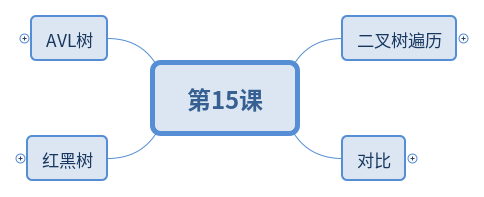
\includegraphics[width=100mm,height=40mm]{images/camp/第15课.png}

\subsubsection{题目}


\subsection{学习总结}

这周我们学习了字典树,并查集,高级搜索,AVL树,红黑树。

字典树的核心思想是空间换时间。利用字符串的公共前缀来降低
查询时间的开销以达到提高效率的目的。

并查集是一个树形结构,用于解决组团、配对问题,判断是否在一个组内。

搜索分为: \\
DFS: depth first search 深度优先搜索,使用栈 \\
BFS: breadth first search 广度优先搜索,使用队列 \\
双向搜索:从起点和终点同时开始 BFS \\
启发式搜索:其实就是使用优先队列,按优先级的高低来搜索

搜索的优化方式: \\
备忘录去重(斐波那契数列) \\
剪枝(生成括号问题)

二叉平衡树的由来:因为二叉树在极端情况下会退化为链表,所以
给二叉树增加了旋转的操作,让二叉树的左右子树保持平衡,这样就不会退化。

四种旋转操作: \\
右右子树:左旋 \\
左左子树:右旋 \\
左右子树:左右旋 \\
右左子树:右左旋

AVL树和红黑树对比: \\
AVL树查询更快,因为AVL树高度平衡,而红黑树是近似平衡。 \\
红黑树插入、删除更快,因为更少的旋转操作。 \\
AVL树每个节点都需要一个整数保存平衡因子,而红黑树只需要一个位来保存红或者黑。

算法学习到第六周了,这周有不少的题目是之前出现过的,
你会发现再次做之前做过的题目,好像好理解很多了。第一次
做的时候,很多东西都是比较晦涩的,而多做了几次之后,情况
就好非常多了。
